% vim: set tw=78 tabstop=4 shiftwidth=4 aw ai:
\documentclass{beamer}

\usepackage[utf8x]{inputenc}		% diacritice
\usepackage[english]{babel}
\usepackage{color}			% highlight
\usepackage{alltt}			% highlight
\usepackage{subfigure}
\usepackage{tikz}
\usepackage{lmodern}
\usepackage[belowskip=-40pt,aboveskip=-2pt]{caption}
\captionsetup{labelformat=empty,labelsep=none}


% highlight; comment this out in case you don't input code source files
%\usepackage{code/highlight}		% highlight

\usepackage{hyperref}			% folositii \url{http://...}
					% sau \href{http://...}{Nume Link}
\usepackage{verbatim}

\mode<presentation>
{ \usetheme{Berlin} }

\newcommand\Wider[2][3em]{%
\makebox[\linewidth][c]{%
  \begin{minipage}{\dimexpr\textwidth+#1\relax}
  \raggedright#2
  \end{minipage}%
  }%
}


% incarcarea simbolurilor Unicode romanesti inn titlu sii primele pagini
\PreloadUnicodePage{200}

\title[Distributed storage and dissemination service based on floating
content]{Distributed storage and dissemination service based on floating
content} 

\subtitle{Analiza fezabilatii stocarii si distributiei de date in
medii mobile, pe baza modelului Floating Content}
% \title[Analiza fezabilatii stocarii si distributiei de date in
% medii mobile, pe baza modelului Floating Content]{Analiza fezabilatii stocarii si distributiei de date in
% medii mobile, pe baza modelului Floating Content}

% \institute{Facultatea de Automatica si Calculatoare,\\
% 	Universitatea POLITEHNICA din Bucuresti}
\institute{
 \begin{tabular}[t]{cc}
Coordonator: Conf.dr.ing. Ciprian Dobre\\
\\
Facultatea de Automatica si Calculatoare,\\
	Universitatea POLITEHNICA din Bucuresti
	\end{tabular}
	}
\author[Mihai Ciocan]{Mihai Ciocan}
\date{Iulie 2014}

\begin{document}

% Slide-urile cu mai multe parti sunt marcate cu textul (cont.)
\setbeamertemplate{frametitle continuation}[from second]

% aratam numarul frame-ului
% \setbeamertemplate{footline}[frame number]

\frame{\titlepage}

\frame{\tableofcontents}

% NB: Sectiunile nu sunt marcate vizual, ci doar apar in cuprins
\section{Stadiul actual si motivatia lucrarii}

% Titlul unui frame se specifica fie in acolade, imediat dupa \begin{frame},
% fie folosind \frametitle
\begin{frame}{Actualitate}
	\begin{itemize}
		\item Se estimeaza ca numarul de utilizatori de device-uri mobile in anul
		2014 va ajunge la 1.75 miliarde (conform eMarketer)
\item Aplicatii utilizate pe device-uri:
		\begin{itemize}
		  \item sociale (Twitter, Facebook, etc.)
		\item comunicatie (WhatsApp, Facebook Messenger) 
		\item localizare, afisare obiective din proximitate, ghidare spatiala(Google
Maps, Waze)
\item combinate (Nearby Friends from Facebook)
\end{itemize}
		\item Majoritatea aplicatiilor sunt dependente de serviciile din
		infrastructura de retea pentru corecta functionare
	\end{itemize}
\end{frame}

\begin{frame}{Posibile probleme}
	\begin{itemize}
	  \item Probleme de conectivitate:
	  \begin{itemize}
	    \item Preturi roaming foarte mari
	  	\item Conectivitate slaba
	  	\item Servicii de date fara acoperire
	  \end{itemize}
	  \item Probleme in managementul datelor transferate:
	  \begin{itemize}
	    \item Relevanta geografica
	    \item Relevanta temporala
	    \item Identificarea detinatorului si pastrarea datelor cu caracter personal
	    \item Utilizarea unui serviciu third-party central de gestiune a datelor
	    poate altera sau cenzura anumite informatii
	  \end{itemize}
	\end{itemize}
\end{frame}

\begin{frame}{Alternativa}
	\begin{itemize}
	  \item Model de distribuire a informatiilor intr-o maniera distribuita
	  (serviciile curente sunt preponderent centralizate)
	  \item Distributia datelor functie de locatie, contextul de comunicatie, 
	  dependent de device-uri mobile situate din vecinatate
	  \item Fiecare utilizator poate genera informatii caracteristice pentru o
	  anumita locatie, pentru o perioda limitata de timp
	  \item Folosind comunicatia intre vehicule, poate fi folosit pentru
	  imbunatatirea experientei de conducere
	  \item Informatii precum: starea vremii, a carosabilului si a traficului
	\end{itemize}
\end{frame}

\section{Modelul aplicatiei}

\begin{frame}{Comportamentul serviciului}
	 \begin{columns}
	    \begin{column}[l]{0.55\textwidth}
			\begin{itemize}
			  \item Fiecare informatie va avea asignata o zona de valabilitate si
			  replicare determinata de razele $a$ si $r$
			  \begin{itemize}
			  \item Informatia distribuita doar vecinilor
			  \item E stearsa atunci cand vehiculul se
			  departeaza 
			  \end{itemize}
			  \item Informatia va ``pluti" (float) atat timp cat exista un numar
			  semnificativ de device-uri in raza de valabilitate pentru a participa la
			  stocare si replicare\ldots oare?
			\end{itemize}
		\end{column}
		\begin{column}[r]{0.45\textwidth}
			\begin{figure}
				\vspace*{-2cm}
				\centering
		    	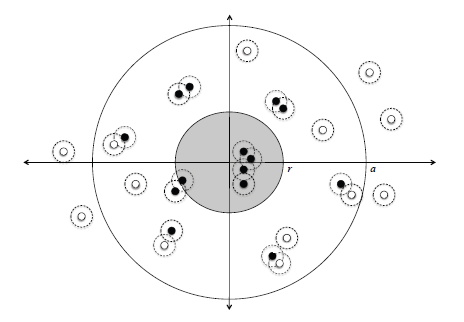
\includegraphics[scale=0.35]{img/anchor_zone}
		    	\caption{Zona gri reprezinta zona de replicare, zona alba este zona
		    	tampon (datele nu se replica, doar se pastreaza)}
		    \end{figure}
		\end{column}
	\end{columns}
\end{frame}

\begin{frame}{Floating Content Protocol}
	Propus de Aalto University, Finland:
	\begin{enumerate}{\fontsize{8}{12}\selectfont
	  \item Nodurile trimit mesaje de descoperire a vecinilor (beacons) la un
	  anumit interval de timp (300s in simulare)
	  \item La primirea unui astfel de mesaj, nodul trimite lista proprie de
	  elemente valabile pentru replicare
	  \item Dupa primirea listei, nodul cere un subset de date, a caror distanta de
	  valabilitate este mai mare decat pozitia nodului fata de origine (nodul se
	  afla in raza de valabilitate)
	  \item Informatiile cerute se transfera pana cand nodurile pierd contactul sau
	  transferul se termina complet
	  \item se repeta pasii incepand de la pasul 1.}
	\end{enumerate}
% 	\begin{itemize}
	Ne propunem sa evaluam fezabilitatea modelului Floating Content,
	impreuna cu protocolul de mai sus, si combinarea originala a acestora
	intr-un serviciu ce ruleaza folosind V2V.
% 	\end{itemize} 
\end{frame}


\section {Criterii propuse de autor pentru evaluarea fezabilitatii}
\begin{frame}{Criterii de fezabilitate - Conditia de criticalitate}
	\begin{itemize}
	  \item $\upsilon$ $\rightarrow$ frecventa cu care un nod intra in contact cu
	  vecinii sai
	  \item $N$ $\rightarrow$ populatia din zona de valabilitate; numarul de
	  perechi este $\frac{1}{2}N(N-1) \approx \frac{1}{2}N^2$; numarul total de
	  contacte este $\frac{1}{2}N^2\upsilon$
	  \item $2p(1-p)$ din numarul de contacte transfera informatie noua unui nod;
	  frecventa acestor evenimente va fi $p(1-p)N^2\upsilon$, frecventa spre care
	  populatia totala ce contine informatia tinde sa creasca;
	  \item $1/\mu$ $\rightarrow$ timpul unui nod aflat in zona de valabilitate;
	  frecventa de iesire a nodurilor din zona este $N\mu$; frecventa de iesire a
	  nodurilor cu informatie este $Np\mu$
	  \item frecventa de crestere este $N\frac{d}{dt}p = N^2p(1-p)\upsilon - Np\mu$
	  \item exista unei solutii pozitive $p^* > 0$ necesita:
	\end{itemize}
	\hskip0.5in
	\small{
		\begin{beamerboxesrounded}[lower=block body,shadow=true,width=3.2in]{}
			\begin{center}
				\texttt{$N\frac{\upsilon}{\mu} > 1$ $\rightarrow$ $criticality\ condition$}
			\end{center}
		\end{beamerboxesrounded}
	}
\end{frame}

\begin{frame}{Criterii de fezabilitate - Modelul epidemic SIR}
	\begin{itemize}
	  \item $S$ $\rightarrow$ noduri ``susceptibile'' (noduri fara informatie), $I$
	  $\rightarrow$ noduri ``infectate'' (detin informatia), $R$ $\rightarrow$ noduri
	  ``vindecate'' (au sters informatia), $r\ \rightarrow$ rata de ``infectare''
	  \mbox{$a$ $\rightarrow$ rata de ``vindecare"}
	  \item $\frac{dS}{dt} = -rSI$ $\rightarrow$ rata de micsorare a numarului de
	  ``susceptibili''
	  \item $\frac{dI}{dt} = rSI - aI$ $\rightarrow$ rata de crestere a numarului
	  de ``infectati''
	  \item $\frac{dR}{dt} = aI$ $\rightarrow$ rata de crestere a numarului de
	  noduri ``vindecate''
	  \item $\left.
\frac{dI}{dt}
\right|_{t=0} = I_{0} (rS_{0} - a)\ \gtrless\ 0\ if\ S_{0}\ \gtrless
\frac{a}{r}\ = \mu$
	\end{itemize}
	\hskip0.5in
	\small{
		\begin{beamerboxesrounded}[lower=block body,shadow=true,width=3.2in]{}
			\begin{itemize}
				\item{$\frac{a}{r}\ = \mu$ $\rightarrow$ $epidemy\ threshold$}
				\item{$S_{0}\ >\ \mu\ \rightarrow$ epidemia este posibila}
				\item{$S_{0}\ <\ \mu\ \rightarrow$ epidemia nu este posibila}
			\end{itemize}
		\end{beamerboxesrounded}
	}
\end{frame}

\section{Rezultate experimentale}

\begin{frame}{Instrumente pentru simulare}
	\begin{columns}[t]
		\begin{column}{0.5\textwidth}
			\begin{itemize}
			  \item Am utilizat framework-ul Veins bazat pe 2 simulatoare
			  \item Simulation of Urban Mobility (road traffic simulator)
			  \item OMNeT++ - simulator de retele
			  \item Cele 2 comunica in timpul simularii prin conexiune TCP
			\end{itemize}
		\end{column}
		\begin{column}{0.5\textwidth}
			\vspace*{-2cm} 
			\begin{figure}
				\centering
				\subfigure{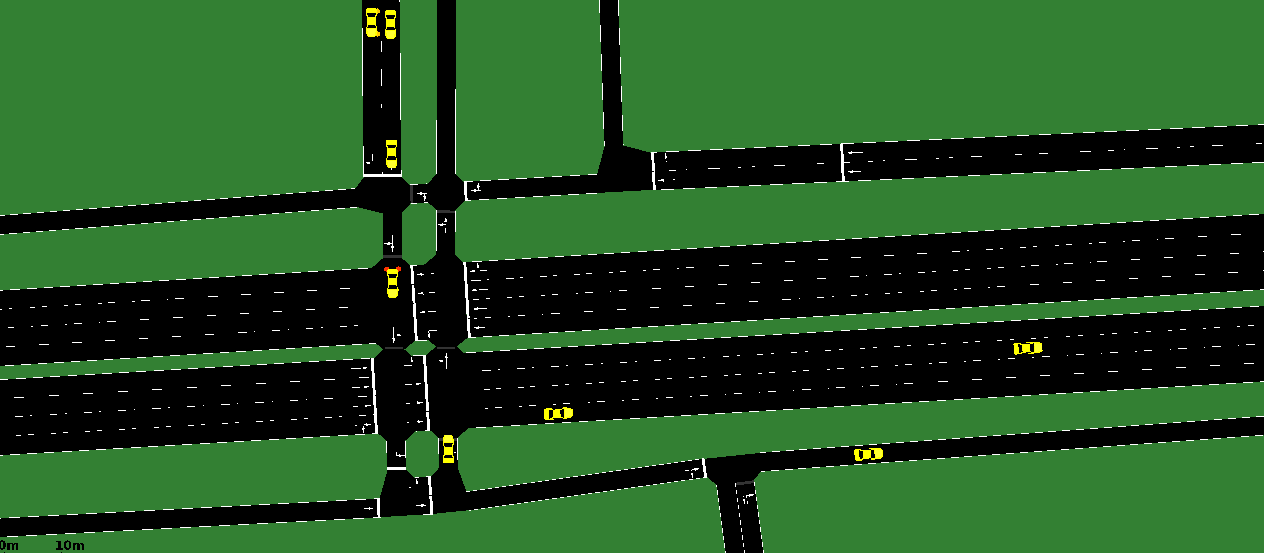
\includegraphics[height=1in]{img/sumo}
				}
				\caption{\tiny SUMO}
			\end{figure}
			\begin{figure}
				\vspace*{0.5cm}
				\centering
				\subfigure{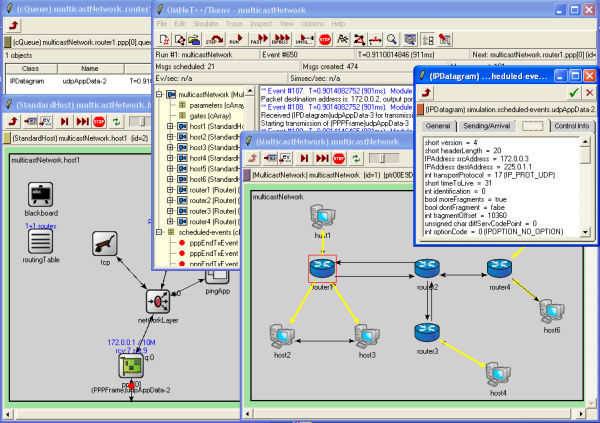
\includegraphics[height=1in, width=2in]{img/omnetpp}
				}
				\caption{\tiny OMNeT++}
			\end{figure}
		\end{column}
	\end{columns}
\end{frame}
\begin{frame}{Colectarea datelor - SanFrancisco}
\Wider{
	\begin{figure}[t]
		\vspace*{-1cm}
		\centering
		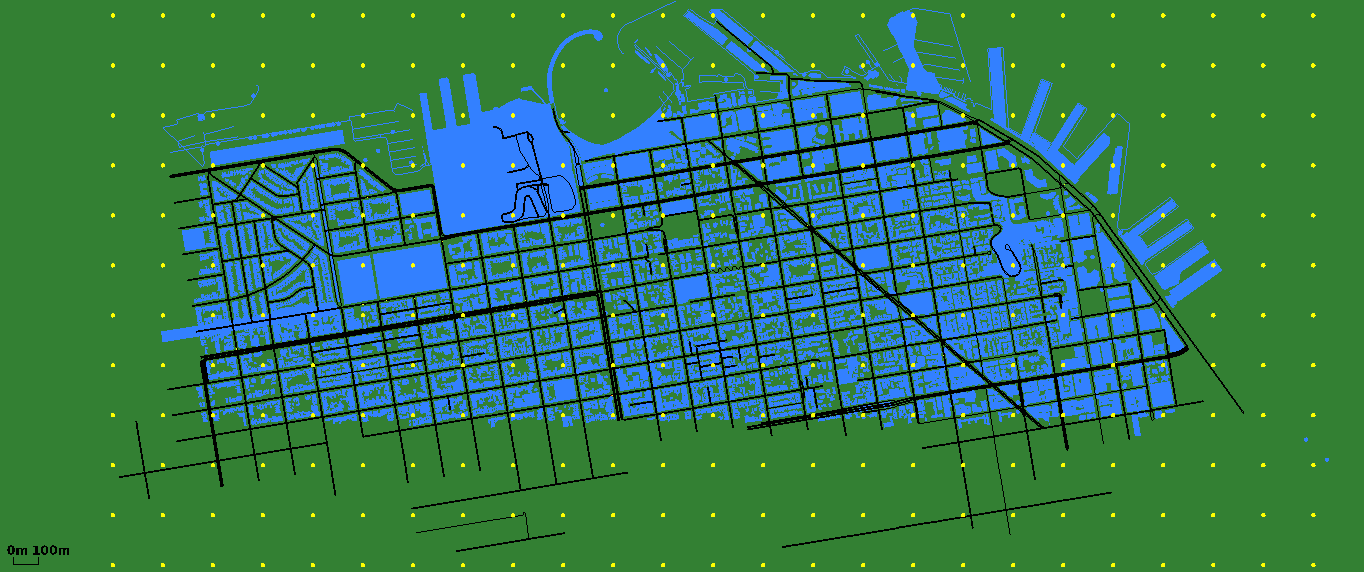
\includegraphics[scale=0.25]{img/SanFrancisco_Anchors}
		\caption{\tiny Punctele semnifica zona de valabilitate a unor elemente
		distincte la distanta de 200m}
	\end{figure}}
\end{frame}

\begin{frame}{Conditia de criticalitate - San Francisco}
	\Wider{
	\begin{figure}[t]
		\vspace*{-1cm} 
		\centering
		\subfigure
		{
\includegraphics[width=2in]{img/SanFrancisco/criticality3_sim_SanFrancisco6_300s_200m}
		
\includegraphics[width=2in]{img/SanFrancisco/avgContacts_sim_SanFrancisco6_300s_200m}
		}
		\caption{\tiny r = 200m}
	\end{figure}
	\begin{figure}[t]
		\centering
		\subfigure
		{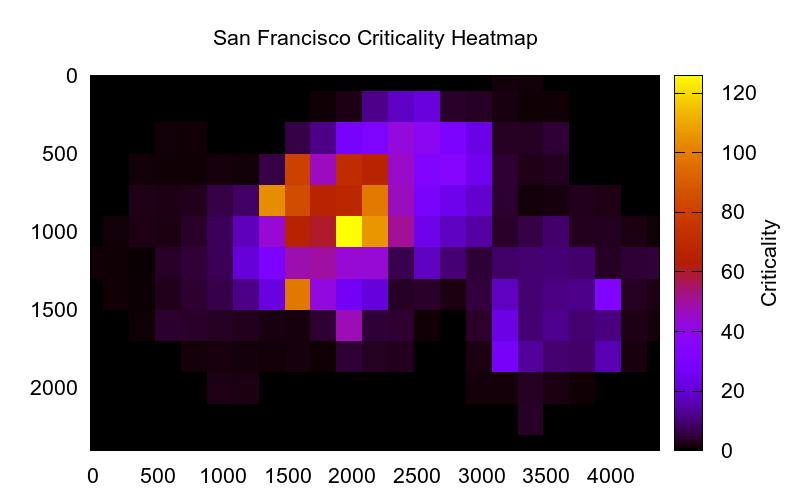
\includegraphics[width=2in]{img/SanFrancisco/criticality3_sim_SanFrancisco6_300s_500m}
		}
		\subfigure
		{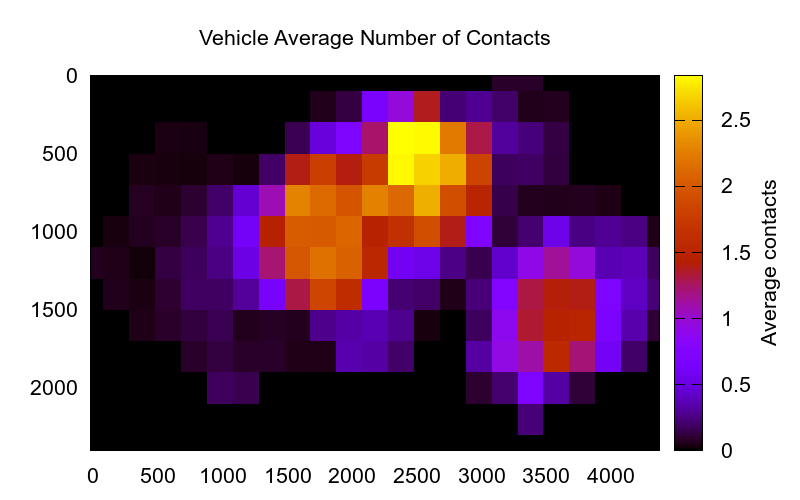
\includegraphics[width=2in]{img/SanFrancisco/avgContacts_sim_SanFrancisco6_300s_500m}
		}
		\caption{\tiny r = 500m}
	\end{figure}
	}
\end{frame}

\begin{frame}{Evolutia numarului de replici a unui element cu r = 500m}
	\begin{figure}[t]
		\centering
		\def\svgwidth{\columnwidth}
		\input{img/SanFrancisco/SanFrancisco500m_epidemic.pdf_tex}
		%\caption{r = 500m, timpul de valabilitate = 600s}
	\end{figure}
	
	\centerline{r = 500m, timpul de valabilitate = 600s}
\end{frame}
\begin{frame}{Evolutia numarului de replici in functie de raza}
	\begin{figure}[t]
		\centering
		\def\svgwidth{\columnwidth}
		\input{img/SanFrancisco/SanFrancisco500m_radii.pdf_tex}
		%\caption{timpul de valabilitate = 600s}
	\end{figure}
	
	\centerline{timpul de valabilitate = 600s}
\end{frame}

\begin{frame}{Concluzii}
	\begin{itemize}
	  \item Am confirmat fezabilitatea modelului de distributie a datelor in
	  mediul urban prin calculul celor 2 criterii
	  \item In ciuda limitarii mobilitatii sintetice, estimam ca modelul va
	  genera in scenarii reale valori mai mici, insa peste pragul de criticalitate
	  necesare raspandirii informatiilor
	  \item In continuarea proiectului, suntem interesati sa intelegem cum se va
	  comporta modelul utilizand memorie limitata si diferite politici de sterge a
	  mesajelor.
	\end{itemize}
\end{frame}
\begin{frame}{Intrebari}
	\begin{figure}
		\centering
		\includegraphics[width=3cm]{img/question_mark}
	\end{figure}
\end{frame}
\end{document}